% SentinelMesh paper, IEEE conference format. Built from paper/writing/paper.md (origin/paper/analysis-writing 038f7e0)
% plus the 2026-10-27 results (E_budget, E9 traces, E1 repeats). Every number cites a file under paper/data/.
% Build: cd paper/ieee && pdflatex paper && pdflatex paper
\documentclass[conference]{IEEEtran}
\usepackage[T1]{fontenc}
\usepackage{amsmath,amssymb}
\usepackage{graphicx}
\usepackage{booktabs}
\usepackage{multirow}
\usepackage{url}
\usepackage{cite}
\usepackage[hidelinks]{hyperref}

\newcommand{\simu}{\textsc{simulated}}
\newcommand{\est}{\textsc{estimated}}
\newcommand{\ph}{\textsc{placeholder}}

\begin{document}

\title{EnergyGate: Defending Battery-Powered IoT Nodes Against Post-Quantum Handshake Exhaustion Attacks}

\author{\IEEEauthorblockN{Ramkiran Garuda}
\IEEEauthorblockA{\textit{School of Computer Science and}\\
\textit{Engineering}\\
\textit{Vellore Institute of Technology}\\
Vellore, India\\
garuda.ramkiran2024@vitstudent.ac.in}
\and
\IEEEauthorblockN{Chaitanya Patil}
\IEEEauthorblockA{\textit{School of Computer Science and}\\
\textit{Engineering}\\
\textit{Vellore Institute of Technology}\\
Vellore, India\\
chaitanya.patil2024@vitstudent.ac.in}
\and
\IEEEauthorblockN{Adithya Binoj Nair}
\IEEEauthorblockA{\textit{School of Computer Science and}\\
\textit{Engineering}\\
\textit{Vellore Institute of Technology}\\
Vellore, India\\
adithya.nair2024@vitstudent.ac.in}}

\maketitle

\begin{abstract}
A battery-powered field device that accepts post-quantum handshakes pays for every request it is asked to check,
whether or not the request is genuine. We measure that cost on commodity ESP32 microcontrollers running ML-KEM
(FIPS~203) and ML-DSA (FIPS~204) over a broadcast ESP-NOW mesh, through a calibrated high-side INA219 rig. At NIST
level~3 the responder's share of one handshake costs $\approx$14.9\,mJ above idle; a forged HELLO carrying a
structurally valid signature forces a full ML-DSA-65 verification ($\approx$3.5\,mJ) before it fails. Over 120\,s
attacks ($n=5$, 95\,\% CI), an undefended insider raises the victim's power by $+91.2\pm3.3$\,mW and cuts
legitimate handshake success to 0.21; a single-signature forger adds $+19.0\pm1.4$\,mW. We present
\emph{EnergyGate}, which decides at the first fragment of a HELLO---before reassembly and before any public-key
work---whether to spend, challenge or drop, using an eight-feature link score and a joule token bucket. It removes
the insider drain ($+1.1$\,mW) without locking out the real gateway, but an attacker that echoes the broadcast
cookie under the \emph{same} (epoch, seq) it was challenged on still drains the victim
($+13.0$\,mW under a cookie that binds to that exact header, down from an unbound cookie's
$+16.0$\,mW; the fix makes the echo dearer for the attacker, not free of cost). The joule budget
is what actually limits this: in 900\,s echo attacks under our gate it empties and admissions
settle near the refill bound $r/c_h=2.5$\,s$^{-1}$, measured extra power falling from
$+12.2\pm4.3$ to $+5.5\pm2.4$\,mW once it does---but only because our placeholder charge
overcosts a forged verify by $\approx$7$\times$; at an honest cost the same bound would sit
above this attacker's own rate and never bind. A slow, one-per-minute attacker evades the score
entirely and never drains the budget either---its own cost is simply too small to matter. Our
defences also protect energy, not availability: the real gateway's success rate tracks the
attacker's frame rate (49\,\% at 100 frames/s) whether or not the victim is spending any crypto
cycles at all. Retrained on recorded traces and evaluated by session, the gate's tree reaches
AUC 0.95 and catches most adaptive traffic the shipped model misses, though the shipped
firmware still carries the original model.
\end{abstract}

\begin{IEEEkeywords}
post-quantum cryptography, ML-KEM, ML-DSA, energy exhaustion, denial of service, ESP32, ESP-NOW, admission control
\end{IEEEkeywords}

%=====================================================================
\section{Introduction}
Post-quantum key exchange is arriving on constrained devices. ML-KEM and ML-DSA~\cite{fips203,fips204} run on a
commodity ESP32 in milliseconds to tens of milliseconds per operation (Table~\ref{tab:e1}), so the question is no
longer whether a microcontroller \emph{can} run a signed post-quantum handshake, but what it costs to let anyone
\emph{ask} it to.

Field devices in distribution grids, pipelines and environmental monitoring often run on a battery and share a
broadcast radio. A post-quantum handshake is an expensive operation, unauthenticated until verified, triggered by a
message anyone in range can send. At NIST level~3 a single HELLO is 4517\,bytes---20 ESP-NOW frames---and checking
it means an ML-DSA-65 verification; admitting it commits the device to an encapsulation, a signature and a 19-frame
response. The cryptography protects the message. Nothing in it protects the battery.

Our motivating scenario follows the 2015 attack on the Ukrainian grid~\cite{ukraine2016}, whose chain ran from
phishing through malicious attachments to the field network and physical access. We study the field-network step:
an attacker within radio range of a battery-powered node who wants to shorten its life or deny service without
breaking any cryptography. Our contributions:
\begin{itemize}
\item \textbf{C1, measured cost.} Energy per post-quantum operation and per handshake on real ESP32 hardware,
through a calibrated INA219 rig, at two parameter sets (Sections~\ref{sec:setup}--\ref{sec:cost}).
\item \textbf{C2, the attack.} Victim power and legitimate-handshake success for six attacker behaviours under
four defences, with five repeats and 95\,\% CIs (Section~\ref{sec:attack}).
\item \textbf{C3, a budget-bounded learned gate.} EnergyGate decides at the first fragment whether to spend,
challenge or drop. We show on the rig that its joule bucket binds at the predicted rate even when the
cookie and the score are both defeated (Sections~\ref{sec:gate}, \ref{sec:attack}, \ref{sec:traces}).
\item \textbf{C4, the artifact.} Firmware, rig description, calibration data, raw logs and scripts that rebuild
every table.
\end{itemize}

%=====================================================================
\section{Background and Related Work}
\textbf{ML-KEM and ML-DSA.} ML-KEM is a module-lattice KEM and ML-DSA a module-lattice signature with
rejection-sampled signing, so its signing time is variable~\cite{fips203,fips204}. We use PQClean's portable C
implementations~\cite{pqclean}.

\textbf{ESP-NOW} is Espressif's connectionless vendor-frame protocol, at most 250\,bytes per frame in v1~\cite{espnow}.
We broadcast, so there is no link-layer retransmission and every station in range hears every frame.

\textbf{PQC cost on small devices.} Gillot \emph{et al.} measure ML-KEM/ML-DSA/SLH-DSA energy on Raspberry Pi and
laptop platforms~\cite{gillot1} and TLS~1.3 PQC handshakes on Pico~W, ESP32 and Pi Zero~\cite{gillot2}; Karcz
\emph{et al.} time the NIST schemes on an ESP32-C6~\cite{karcz}. All characterise the cost the device \emph{wants} to
pay. None measures the cost an adversary chooses when to impose.

\textbf{Handshake exhaustion.} Lee \emph{et al.} show PQC-TLS prolongs high server CPU load under handshake
exhaustion by up to 88$\times$ and degrades learned IDSs~\cite{leetls}---server CPU, not battery. Hummen \emph{et al.}
protect constrained peers' public-key work with puzzles~\cite{hummen}; client puzzles and cookies for key exchange
are well studied~\cite{stebila,rfc8019}. On a broadcast medium a stateless cookie only stops blind spoofers.

\textbf{Battery exhaustion.} Stajano and Anderson named ``sleep deprivation torture''~\cite{stajano};
Pirretti \emph{et al.} analyse sleep-deprivation attacks in sensor networks~\cite{pirretti}. Those defences sit at
the MAC/clustering layer. From a first, non-systematic search (\texttt{paper/writing/related\_work.md}) we found no
prior measurement of the battery cost of abusive post-quantum handshake requests on a microcontroller and no defence
that bounds it with a joule budget independent of a classifier; we do not claim this is exhaustive.

%=====================================================================
\section{Threat Model}
\textbf{Setting.} One battery-powered responder (\emph{field-1}) and one mains-powered gateway (the initiator) share
a broadcast ESP-NOW channel. Only the gateway initiates; a real field node never sends a HELLO.

\textbf{Attacker.} Within radio range; transmits arbitrary frames at any rate; holds no legitimate long-term key;
spoofs any sender id (ESP-NOW frames are unauthenticated); hears every frame, so it can replay HELLOs and echo any
broadcast cookie; and knows the defence, its features, thresholds and budget (Kerckhoffs). Behaviours:
\begin{itemize}
\item \textbf{FLOOD}: forged HELLOs under the gateway's id with random signature bytes. ML-DSA rejects them during
signature unpacking ($\approx$1.7\,ms), so they are cheap to reject.
\item \textbf{FORGE}: one \emph{structurally valid} ML-DSA-65 signature from the attacker's own key, resent under
the gateway's id with fresh (epoch, seq). It passes unpacking, so field-1 runs the full verification and fails only
at the end. One attacker signature forces a full check on every resend.
\item \textbf{INSIDER}: HELLOs validly signed with an \emph{enrolled} key (a compromised peer); each admitted HELLO
costs a full responder handshake.
\item \textbf{SLOW\_DRIP}: INSIDER at $\approx$1 HELLO/min, below any fixed rate limit.
\item \textbf{ADAPTIVE / ADAPTIVE\_SPOOF}: knows EnergyGate's features; keeps \texttt{hs\_fail} and \texttt{dup\_pct}
at zero and paces \texttt{hs\_per\_s} under the tree's split with AIMD back-off on a heard CHALLENGE.
\item \textbf{+ECHO}: any of the above, also echoing the cookie from each CHALLENGE it hears.
\end{itemize}
\textbf{Out of scope:} jamming, physical capture, side channels, breaking ML-KEM/ML-DSA. The attacker wins by
maximising victim energy or denying the gateway a session; we report both.

%=====================================================================
\section{System: the Post-Quantum Handshake}
A signed-KEM exchange in three messages, on PQClean (commit \texttt{0586a824}):
\begin{align*}
I\!\to\! R:&\ \textsf{HELLO}=\text{cookie}\,\|\,n_i\,\|\,pk_{\mathrm{KEM}}\,\|\,\sigma_I(\text{th}_1)\\
R\!\to\! I:&\ \textsf{RESPONSE}=n_i\,\|\,n_r\,\|\,ct\,\|\,\sigma_R(\text{th}_2, R, I)\\
I\!\to\! R:&\ \textsf{CONFIRM}=n_r\,\|\,\text{tag}
\end{align*}
with $\text{th}_1=\text{XOF}(I,R,n_i,pk)$, $\text{th}_2=\text{XOF}(\text{th}_1,n_r,ct)$, session keys
$\text{XOF}(ss,\text{th}_2)$ and SHAKE256 as XOF. Static provisioned ML-DSA keys authenticate; an ephemeral ML-KEM
key agrees. Session keys drive AES-256-GCM. The cookie lies outside the signed transcript so that, after a
CHALLENGE, the initiator resends the same signed HELLO without signing again. The protocol is host-tested against
forged signatures, wrong keys, tampered fields and replays, but \textbf{not formally verified}.

Level~1 is ML-KEM-512 + ML-DSA-44; level~3 (default) is ML-KEM-768 + ML-DSA-65. Level~5 does not fit: ML-DSA-87
signing needs more stack than the largest free heap block (110\,580\,B). Table~\ref{tab:sizes} gives message sizes.

\begin{table}[t]
\caption{Message sizes and ESP-NOW frames (235\,B payload per frame)}
\label{tab:sizes}
\centering\small
\begin{tabular}{lccc}
\toprule
Level & HELLO & RESPONSE & CONFIRM\\
\midrule
1 & 3244\,B, 14 fr. & 3220\,B, 14 fr. & 48\,B, 1 fr.\\
3 & 4517\,B, 20 fr. & 4429\,B, 19 fr. & 48\,B, 1 fr.\\
\bottomrule
\end{tabular}
\end{table}

\textbf{Resource bounds.} The reassembler tracks at most 8 streams with a 3\,s timeout. All post-quantum work runs in
one task with a reserved stack (90\,112\,B at level~3); while busy, admissions are refused (\texttt{busy\_drop}),
which caps the crypto rate. \textbf{Replay guard:} per sender, the last 8 verified epochs with their highest
verified sequence number; unverified HELLOs never advance it.

%=====================================================================
\section{EnergyGate}\label{sec:gate}
\textbf{Placement.} On field-1, whose battery is at risk. Inbound HELLO checks run: header sanity, replay/freshness,
allow-list, EnergyGate with the joule budget, then reassembly and ML-DSA verification. EnergyGate decides on the
\emph{first fragment}. DROP is silence; the radio still receives the remaining fragments, and that residual cost is
measured, not assumed away.

\textbf{Score.} A depth-4 decision tree, exported to C, maps eight link features over a rolling 5\,s window to the
probability that the sender is genuine: \texttt{hs\_per\_s}, \texttt{hs\_fail}, \texttt{rssi\_mean},
\texttt{rssi\_var}, \texttt{loss\_pct}, \texttt{dup\_pct}, \texttt{frag\_complete\_pct}, \texttt{battery\_pct}.
The shipped model was trained on \simu{} traces.

\textbf{Joule budget.} A token bucket of capacity $B$ refilling at $r$\,J/s; an admitted handshake is charged $c_h$,
a challenge $c_c$. Every run used the \ph{} values $B=20$\,J, $r=0.05$\,J/s, $c_h=0.02$\,J, $c_c=0.5$\,mJ. Measured
values (Section~\ref{sec:cost}): field-1's share of a handshake is $\approx$14.9\,mJ (so $c_h$ overcharges it by
1.3$\times$), a failed FORGE verify $\approx$3\,mJ measured directly ($14.7$\,mW$/4.97$\,s$^{-1}$,
Section~\ref{sec:attack}; $7\times$ overcharge), and $c_c\lesssim0.4$\,mJ (an upper bound from the noise floor).
Since the bucket never spends more than it holds,
\begin{equation}
\textstyle\sum_{\text{admits in }[0,T]} c \;\le\; B + rT,
\qquad \lim_{T\to\infty}\bar P_{\text{charged}} \le r,
\label{eq:bound}
\end{equation}
for \emph{any} admission sequence, whatever the score says. It caps what is \emph{charged}; it caps real drain only
when $c_h$ is at least the true cost, and it does not cover reception of frames before the gate decides.

\textbf{Policy v2} (default), with score $p$, thresholds 0.7/0.4: (1)~$p\ge0.7$ and budget covers $c_h$ $\to$ SPEND;
(2)~a valid cookie returned and budget covers $c_h$ $\to$ SPEND whatever the score; (3)~budget cannot cover one
handshake $\to$ DROP; (4)~$p\ge0.4\to$ CHALLENGE; (5)~otherwise CHALLENGE charged $c_c$, DROP only if $c_c$ cannot
be paid. \textbf{Policy v1} (ablation) drops at rule~5 and needs $p\ge0.4$ at rule~2.

\textbf{Baselines.} NONE; RATELIMIT (one admission per sender per 10\,s); COOKIE (challenge every sender until it
echoes a cookie; no model, no budget).

%=====================================================================
\section{Measurement Setup}\label{sec:setup}
Four ESP32-WROOM-32 devkits (ESP32-D0WD-V3, 240\,MHz): field-1 (victim), gateway, attacker, monitor. PlatformIO
6.2.0, espressif32 7.1.3. Energy builds strip the demo peripherals. There is no battery: \texttt{battery\_pct} is
fixed at 100 (\simu).

\textbf{Rig.} Field-1 is powered from a 5\,V adaptor \emph{only} through a high-side INA219 (0.1\,$\Omega$ shunt,
0.1\,mA/bit), read by the monitor at $\approx$989\,samples/s over 400\,kHz I$^2$C. Field-1 raises GPIO4 around each
measured operation; the monitor reports per-interval duration, energy and peak current, and a true 1\,s mean power.

\textbf{Calibration.} Seven loads from 0 to 232\,mA against a DT830D multimeter fit
$I_{\mathrm{INA}}=1.0367\,I_{\mathrm{ref}}-0.428$\,mA; after correction residuals are within 0.6\,\% over
57--232\,mA and $\approx$0.17\,mA below 20\,mA. Systematics are quoted separately: the 3.67\,\% gain difference
between the two instruments is unresolved and affects absolute joules (C1) but cancels in ratios. Raw logs stay
uncorrected; correction is applied in analysis.

\textbf{Method note.} The monitor's instantaneous current sample aliases against a 5\,Hz attacker (one FORGE run read
$\approx$0\,mW, another $+125$\,mW). All power results use the 1\,s mean.

\begin{table}[t]
\caption{Primitive timings, radio off (ms; median of four boards, 5 sessions each; signing pooled, $n=116$)}
\label{tab:e1}
\centering\small
\setlength{\tabcolsep}{3pt}
\begin{tabular}{lccc}
\toprule
Algorithm & keygen & encaps/sign & decaps/verify\\
\midrule
ML-KEM-512 & 5.93 & 6.05 & 7.35\\
ML-KEM-768 & 8.59 & 9.88 & 11.60\\
ML-KEM-1024 & 13.14 & 14.37 & 16.46\\
ML-DSA-44 & 15.36 & 48.8 (p10 24.1, p90 92.4) & 15.97\\
ML-DSA-65 & 26.00 & 63.4 (p10 37.1, p90 152.7) & 26.25\\
X25519$^\dagger$ & 397.45 & 403.76 & ---\\
ECDSA-P256$^\dagger$ & 191.16 & 89.04 & 202.56\\
\bottomrule
\end{tabular}\\[2pt]
{\footnotesize $^\dagger$mbed TLS generic C; not a fair PQC-vs-classical comparison.}
\end{table}

%=====================================================================
\section{Results: Cost of the Handshake (C1)}\label{sec:cost}
Deterministic timings agree across all four boards within 0.6\,\% (Table~\ref{tab:e1}); signing is rejection-sampled,
so we report its pooled distribution (ML-DSA-65 max 394.8\,ms). Table~\ref{tab:e2} gives energy per operation
(radio off, $n=20$ per op; idle 225\,mW).

\begin{table}[t]
\caption{Energy per operation, radio off (mean, $n=20$). ``Above idle'' subtracts 225\,mW $\times$ duration}
\label{tab:e2}
\centering\small
\begin{tabular}{lccc}
\toprule
Operation & ms & total mJ & above idle mJ\\
\midrule
ML-KEM-768 keygen & 8.6 & 2.91 & 0.98\\
ML-KEM-768 encaps & 9.7 & 3.27 & 1.10\\
ML-KEM-768 decaps & 11.5 & 3.93 & 1.34\\
ML-DSA-44 sign & 44 & 15.4 & 5.4 $\pm$ 1.3\\
ML-DSA-44 verify & 16.2 & 5.57 & 1.93\\
ML-DSA-65 keygen & 26.0 & 9.05 & 3.19\\
ML-DSA-65 sign & 86 & 30.0 & 10.6 $\pm$ 4.1\\
ML-DSA-65 verify & 26.2 & 9.14 & 3.23\\
X25519 shared secret$^\dagger$ & 476 & 150 & 43.3\\
ECDSA-P256 sign$^\dagger$ & 115 & 36 & 9.9\\
\bottomrule
\end{tabular}
\end{table}

At level~3, field-1's share of a handshake is verify + encaps + sign $= 3.23+1.10+10.6\approx\mathbf{14.9}$\,mJ above
idle; both sides together cost $\approx$31\,mJ. On the live mesh with the radio always on (field-1 idles at
$\approx$598\,mW), one legitimate handshake costs 9--65\,mJ above idle (80--560\,ms, dominated by signing variance);
one admitted FORGE HELLO $\approx$3.45\,mJ per marked operation; one admitted FLOOD HELLO is not measurably different
from zero. Peak crypto current is $\approx$71\,mA. The idle radio dominates absolute drain, so any battery-life
claim depends on a duty-cycle assumption we state rather than hide: our victim never sleeps.

%=====================================================================
\section{Results: Attacks and Defences (C2, C3)}\label{sec:attack}
Each cell of Table~\ref{tab:e5} attacks for 120\,s at 5\,HELLO/s (SLOW\_DRIP: $\approx$1/min). Extra power is
field-1's mean power over the attack minus the minute before; $n=5$, 95\,\% CI. Legit success is the gateway's
completed/started handshakes during the attack.

\begin{table}[t]
\caption{E5 energy grid: extra victim power and legitimate success}
\label{tab:e5}
\centering\small
\setlength{\tabcolsep}{2pt}\footnotesize
\begin{tabular}{llcc}
\toprule
Defence & Attack & Extra power (mW) & Legit success\\
\midrule
\multirow{6}{*}{none} & FLOOD & $+1.8\pm2.2$ & $0.71\pm0.23$\\
 & \textbf{INSIDER} & $\mathbf{+91.2\pm3.3}$ (+15.2\,\%) & $0.21\pm0.15$\\
 & SLOW\_DRIP & $+0.2\pm0.6$ & $0.96\pm0.11$\\
 & \textbf{FORGE} & $\mathbf{+19.0\pm1.4}$ (+3.2\,\%) & $0.28\pm0.24$\\
 & \textbf{ADAPTIVE} & $\mathbf{+28.9\pm2.3}$ & $0.30\pm0.30$\\
 & ADAPT.\_SPOOF & $-0.4\pm1.8$ & $0.65\pm0.64$\\
\midrule
ratelimit & FLOOD/INS./DRIP & $-2.2/-1.4/+0.4$ & \textbf{0.00}/0.87/0.81\\
\midrule
\multirow{2}{*}{cookie} & FLOOD/INS./DRIP & $+1.8/+1.4/-0.1$ & 0.79/0.77/1.00\\
 & FORGE/AD./A.S. & $+0.8/+1.2/-1.4$ & 0.24/0.53/0.52\\
\midrule
\multirow{3}{*}{gate v2} & FLOOD/INS./DRIP & $+1.7/+1.1/+0.7$ & 0.75/0.82/1.00\\
 & FORGE/A.S. & $+1.4/-0.4$ & 0.23/0.47\\
 & \textbf{ADAPTIVE} & $\mathbf{+25.5\pm3.0}$ & $0.45\pm0.33$\\
\midrule
gate v1 & FLOOD/INSIDER & $-2.6/-3.0$ & \textbf{0.04/0.02}\\
\bottomrule
\end{tabular}
\end{table}

\textbf{Findings.} (i)~FORGE, not FLOOD, is the cheap-attacker/costly-victim attack: one attacker signature forces a
$\approx$3.5\,mJ verify per resend, while random signatures cost nothing measurable. (ii)~INSIDER is the largest
undefended drain and starves the gateway; every defence removes the drain, but RATELIMIT does so by also locking out
the gateway under FLOOD (0\,\%). (iii)~Gate~v1 locks out the gateway (2--4\,\%): forged and real HELLOs share a
sender id and look alike to window features, so dropping low scores drops both. Gate~v2's cookie rule fixes that.
(iv)~ADAPTIVE evades the score and still drains $+25.5$\,mW under gate~v2. (v)~In a rate sweep (5/20/50\,s$^{-1}$,
$n=3$) INSIDER's undefended drain is flat ($+94$ to $+96$\,mW) because the single crypto slot saturates at 5/s; the
gate holds it near $+1.5$\,mW at every rate. A fast FLOOD costs no energy but drops legit success from $\approx$0.5
to $\approx$0.07 through airtime and reassembly contention---a different denial than the energy one. (vi)~A 30-min
SLOW\_DRIP shows no measurable extra power.

\textbf{FORGE + ECHO (original run, unbound cookie) drew $+15.1\pm2.4$\,mW under COOKIE and $+16.0\pm0.5$\,mW
under gate~v2} ($n=5$), $\approx$540 forged HELLOs spent per run, legit success $\approx$0.13. The cookie as built
then was \emph{reusable}: bound to neither the HELLO's nonce nor its (epoch, seq), so $\approx$30 echoes admitted
every later resend of the cached template, and gate~v2's rule~2 let them through on top of that.

\textbf{The cookie now binds to (sender, epoch, seq, window); the fix makes a real echo dearer, not free.} Binding
it closes the \emph{reuse}, but a first attempt broke the real gateway too---its own cookie retry also used a fresh
seq, so a bound cookie never verified for it either. Fixed by having the gateway keep the challenged (epoch, seq)
on retry, and by giving the attacker an \texttt{ECHO same} mode that does the same (real echo, not the old
bug). Rerun on the INA219 (53 runs, firmware \texttt{7afdea4}, Table~\ref{tab:cookiefix}): with no attack the real
gateway now gets in 128/132 times. COOKIE stops a non-echoing or fresh-seq attacker (within $\approx$1\,mW of
idle, against $+14.7\pm0.9$\,mW undefended). A same-seq echo is \emph{not} stopped: $+13.0\pm1.0$\,mW over 900\,s,
$\approx$12\,\% below undefended, at the cost of one echo per HELLO ($\approx$4.7\,s$^{-1}$, roughly double the
frames) instead of $\approx$30 cheap echoes per run. \textbf{Dearer for the attacker, not closed, little saved
for the victim.}

\begin{table}[t]
\caption{Cookie-fix rerun, 900\,s windows, INA219 rig (except control)}
\label{tab:cookiefix}
\centering\small
\begin{tabular}{llcc}
\toprule
Defence & Attacker & Extra power & Admits/s\\
\midrule
none & none (control) & $+0.2\pm0.4$\,mW & --\\
none & FORGE, no echo (120\,s) & $+14.7\pm0.9$\,mW & 4.97\\
cookie & \texttt{ECHO same} & $\mathbf{+13.0\pm1.0}$\,mW & 4.71\\
gate v2 & \texttt{ECHO same} & $+12.2\pm4.3 \to \mathbf{+5.5\pm2.4}$\,mW & $4.50\to2.42$\\
\bottomrule
\end{tabular}
\end{table}

\textbf{The joule budget, not the cookie or the score, is what limits a same-seq echo under gate~v2---and this is
now measured, not estimated.} Three 900\,s \texttt{ECHO same} runs against gate~v2 (Fig.~\ref{fig:budget},
Table~\ref{tab:budget}; the first such test, on USB with no INA219 and the old reusable cookie, already showed
admissions settle at 2.48--2.49\,s$^{-1}$ $=r/c_h$ once a 600\,s attack ran the bucket dry at $+537$\,s) each ran
the bucket dry ($+412$ to $+633$\,s) and admissions settled at 2.42\,s$^{-1}$, again near the refill bound. Extra
power fell from $+12.2\pm4.3$\,mW before exhaustion to $\mathbf{+5.5\pm2.4}$\textbf{\,mW, measured}, after---this
\textbf{replaces} the earlier $\approx8.6$\,mW \est{} figure, which had no power reading at all. COOKIE has no
budget and stays flat at $+13.0$\,mW for as long as the attack runs; the first few minutes of the gate~v2 run show
no advantage over COOKIE either, until the bucket actually empties.

\textbf{This bound only binds because $c_h$ is a placeholder.} A forced verify really costs $\approx$3\,mJ
($14.7$\,mW$/4.97$\,s$^{-1}$), not the $c_h=20$\,mJ charged---an overcharge of $\approx7\times$. At an honest
$c_h$, the sustainable rate $r/c_h\approx16.7$\,s$^{-1}$ would exceed this attacker's own $\approx5$\,s$^{-1}$, and
the bucket would never empty: this follows from (\ref{eq:bound}) and the already-measured rates, with no further
experiment needed. We report this rather than silently relying on it: the bound demonstrated above holds
\emph{here} because of how the placeholder overcharges, not in general.

\textbf{Defences protect energy, not availability.} The real gateway's success rate tracks the attacker's frame
rate, not field-1's crypto load: 49\,\% at 100 forged frames/s whether field-1 verifies every one (no defence) or
none (COOKIE/gate with no echo), and 8--21\,\% once the attacker echoes. Consistent with frame loss under radio
load, though no frame-level loss was measured directly. Neither COOKIE nor gate~v2 restores availability in these
runs; both recover within the attack's last minute once it stops.

\begin{figure}[t]
\centering
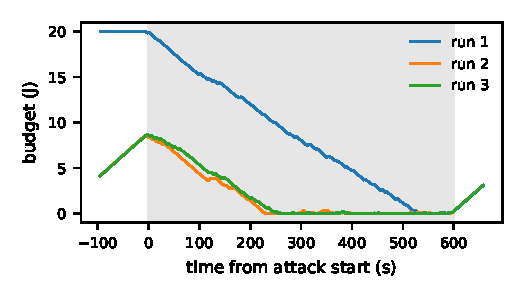
\includegraphics[width=\columnwidth]{fig_budget.pdf}
\caption{Field-1's joule budget during three 600\,s FORGE+ECHO attacks (shaded) under gate v2. Once empty,
admissions are pinned to the refill rate.}
\label{fig:budget}
\end{figure}

\begin{table}[t]
\caption{Budget runs: FORGE+ECHO, 600\,s, gate v2}
\label{tab:budget}
\centering\small
\begin{tabular}{lccccc}
\toprule
Run & start & empty at & spend/s before & after & drop/s after\\
\midrule
1 & 20.0\,J & +537\,s & 4.52 & \textbf{2.48} & 2.20\\
2 & 8.6\,J & +235\,s & 4.13 & \textbf{2.49} & 1.79\\
3 & 8.6\,J & +260\,s & 4.10 & \textbf{2.49} & 2.17\\
\bottomrule
\end{tabular}
\end{table}

%=====================================================================
\section{EnergyGate on Recorded Traces}\label{sec:traces}
The shipped tree was trained on \simu{} traces. We recorded field-1's own eight features and the carried score once a
second (6 attacks $\times$ 3 sessions plus the 3 budget runs; $\approx$7\,800 rows) and evaluated
\emph{leave-one-session-out}---never randomly, since neighbouring rows share a 5\,s window. Transition rows are
excluded; \texttt{battery\_pct} is constant and dropped. RSSI is 0 when no HELLO arrived, so it can leak ``any HELLO =
attack''; we report with and without it (Table~\ref{tab:e9}).

\begin{table}[t]
\caption{Attack detection, leave-one-session-out (6 folds). Detection rates at score threshold 0.5}
\label{tab:e9}
\centering\small
\setlength{\tabcolsep}{2pt}\footnotesize
\begin{tabular}{lcccccc}
\toprule
Model & AUC & TPR@1\% & FPR & DRIP & ADAPT. & A.SP.\\
\midrule
carried (\simu) & 0.876 & 0.751 & 0.000 & 0.00 & 0.00 & 0.00\\
rate rule & 0.905 & 0.809 & 0.000 & 0.00 & 0.82 & 0.06\\
tree, 7 feat. & 0.935 & 0.881 & 0.014 & 0.05 & 0.93 & 0.74\\
tree, no RSSI & \textbf{0.950} & \textbf{0.903} & 0.008 & 0.07 & 0.97 & 0.86\\
\bottomrule
\end{tabular}
\end{table}

The carried \simu-trained model flags FLOOD, INSIDER, FORGE and FORGE+ECHO perfectly with no false alarms, but misses
SLOW\_DRIP, ADAPTIVE and ADAPTIVE\_SPOOF entirely. Retraining on recorded traces lifts AUC to 0.95 and catches most
adaptive traffic; dropping RSSI \emph{helps}, consistent with the leak. SLOW\_DRIP stays essentially invisible
(7\,\%) to every model. All sessions come from one rig, one room and one distance, so a held-out session is not a
held-out environment. The honest reading is C3's: the classifier is evadable; the budget is the guarantee.

%=====================================================================
\section{Limitations}
\begin{itemize}
\item \textbf{No battery}: a 5\,V adaptor stands in; battery figures are derived from joules, and the victim's radio
never sleeps.
\item \textbf{Placeholder budget, shown to matter}: every run used $c_h=20$\,mJ, $\approx7\times$ a forged verify's
real $\approx$3\,mJ cost; at the honest cost the bound's sustainable rate ($\approx$16.7\,s$^{-1}$) exceeds this
attacker's own ($\approx$5\,s$^{-1}$), so it would not have bound at all. Measured costs are not yet written back.
\item \textbf{Attacker energy} is not measured (no second monitor), so the victim-to-attacker energy ratio of C2 is
still outstanding; we report victim power only.
\item \textbf{Cookie reuse, fixed and rerun}: the original cookie bound to neither the HELLO's nonce nor its
(epoch, seq); the fix (Section~\ref{sec:attack}) makes a real echo dearer, not free, and a first version of it
locked out the legitimate gateway until the gateway's own retry was corrected to match.
\item \textbf{Defences protect energy, not availability}: the real gateway's success tracked the attacker's frame
rate, not field-1's crypto load, in every rerun condition (Section~\ref{sec:attack}).
\item \textbf{Shipped model is still \simu{}-trained}: Section~\ref{sec:traces}'s retrain is not exported to firmware,
so every power result here used the original model.
\item \textbf{Absolute energy} rests on an unresolved 3.67\,\% instrument gain difference; ratios are unaffected.
\item \textbf{Unauthenticated control channel}, demo keys compiled into images, no formal verification, no level~5,
one chip family, one victim and one legitimate peer; legit-success CIs are wide (few handshakes per window).
\item \textbf{Replay ring}: a captured HELLO whose epoch aged out of the 8-entry ring can be replayed once.
\item \textbf{Budget runs}: the first (USB, no INA219) measured counters, not power; the second (INA219, bound
cookie) measured power directly and replaces its $\approx$8.6\,mW \est{} figure with $+5.5\pm2.4$\,mW measured.
\end{itemize}

%=====================================================================
\section{Conclusion}
On a battery-powered post-quantum responder the battery, not the message, is the attack surface: an enrolled
insider raises the victim's power by 15\,\% and a single forged signature, resent, forces a full ML-DSA verify every
time. A first-fragment gate removes most of the damage cheaply, but a learned score is evadable, and binding the
broadcast cookie to the exact HELLO it answers makes a real echo dearer rather than free. The joule budget is the
part that does not depend on being right about the attacker or the cookie: on the rig it pinned admissions to
$r/c_h$ and cut a same-seq echo's drain from $+12.2$ to $+5.5$\,mW once it ran dry---but only because our
placeholder cost overcharges a forged verify by $\approx7\times$; at an honest cost the same attacker would never
have drained it. Our defences also protect energy, not availability: the gateway's success tracked the attacker's
frame rate regardless of which defence ran. Next steps are an honestly-costed budget (with $r$ set from a target
battery life), deploying the retrained gate, a second monitor for attacker energy, and a duty-cycled victim.

\section*{Artifact}
\texttt{firmware/} (all board firmware, host tests), \texttt{ml/} (EnergyGate training/export),
\texttt{paper/data/} (raw logs, never edited; \texttt{paper/runlog.csv} lists every run, excluded ones marked),
\texttt{paper/analysis/} (scripts rebuilding every table, including \texttt{e9\_retrain.py} and
\texttt{fig\_budget.py}).

\begin{thebibliography}{99}
\bibitem{fips203} NIST, ``Module-Lattice-Based Key-Encapsulation Mechanism Standard,'' FIPS 203, Aug. 2024.
\bibitem{fips204} NIST, ``Module-Lattice-Based Digital Signature Standard,'' FIPS 204, Aug. 2024.
\bibitem{pqclean} M. J. Kannwischer \emph{et al.}, ``Improving software quality in cryptography standardization
projects,'' in \emph{Proc. IEEE EuroS\&P Workshops}, 2022. (PQClean.)
\bibitem{espnow} Espressif Systems, ``ESP-NOW,'' ESP-IDF Programming Guide.
\bibitem{ukraine2016} R. M. Lee, M. J. Assante, and T. Conway, ``Analysis of the cyber attack on the Ukrainian power
grid,'' SANS ICS / E-ISAC, Mar. 2016.
\bibitem{gillot1} Gillot, Buchanan, and Tehrani, ``Energy consumption of post-quantum cryptography on constrained and
general-purpose architectures,'' \emph{Cryptography}, vol. 10, no. 4, 2026.
\bibitem{gillot2} Gillot, Buchanan, and Turino, ``Testing TLS 1.3 PQC on constrained devices and
microcontrollers,'' arXiv:2610.27766, 2026.
\bibitem{karcz} Karcz, Niemiec, Kourtis, and K\"oppl, ``Exploring hardware implementation feasibility of
post-quantum cryptography in embedded systems: ML-KEM, ML-DSA and SLH-DSA on ESP32-C6,'' \emph{PLOS ONE}, 2026.
\bibitem{leetls} Lee, Chang, Yu, and Yeh, ``On the security implications of PQC in TLS: handshake exhaustion and IDS
degradation,'' arXiv:2607.12504, 2026.
\bibitem{hummen} R. Hummen, H. Wirtz, J. H. Ziegeldorf, J. Hiller, and K. Wehrle, ``Tailoring end-to-end IP security
protocols to the Internet of Things,'' in \emph{Proc. IEEE ICNP}, 2013.
\bibitem{stebila} D. Stebila, L. Kuppusamy, J. Rangasamy, C. Boyd, and J. Gonzalez Nieto, ``Stronger difficulty
notions for client puzzles and denial-of-service-resistant protocols,'' in \emph{CT-RSA}, 2011.
\bibitem{rfc8019} Y. Nir and V. Smyslov, ``Protecting Internet Key Exchange Protocol Version 2 (IKEv2) implementations
from distributed denial-of-service attacks,'' RFC 8019, 2016.
\bibitem{stajano} F. Stajano and R. Anderson, ``The resurrecting duckling: security issues for ad-hoc wireless
networks,'' in \emph{Security Protocols Workshop}, 1999.
\bibitem{pirretti} M. Pirretti \emph{et al.}, ``The sleep deprivation attack in sensor networks: analysis and methods
of defense,'' \emph{Int. J. Distrib. Sensor Netw.}, vol. 2, no. 3, pp. 267--287, 2006.
\end{thebibliography}

\end{document}
